\section{模型描述}
\subsection{标准化与传统分类器}
为消除特征尺度差异，对人工特征第 $j$ 维执行
\begin{equation}
 z_{ij}=\frac{x_{ij}-\mu_j}{\widetilde\sigma_j},\qquad
 \widetilde\sigma_j=\begin{cases}\sigma_j,&\sigma_j>0,\\1,&\sigma_j=0.\end{cases}
\end{equation}
均值和标准差仅由当前训练部分估计。逻辑回归使用多类线性判别与交叉熵拟合，$C$ 控制正则化强度的倒数。SVM 采用径向基核 $K(\boldsymbol{z},\boldsymbol{z}')=\exp(-\gamma\|\boldsymbol{z}-\boldsymbol{z}'\|_2^2)$，调整 $C$ 与 $\gamma$\cite{cortes1995}。随机森林集成 200 棵树，调整树深度及叶节点最小样本数，不额外执行标准化\cite{breiman2001}。

另以固定 $C=0.1$ 的逻辑回归考察主成分分析（PCA）。在每折训练部分内拟合标准化器与 PCA，再变换验证数据；分别保留 90\%、95\% 和 99\% 的累计解释方差。PCA 以方差保留为目标，并不直接最大化类别可分性\cite{jolliffe2016}，因此降维后的分类效果需要通过实验判断。

\subsection{单分支神经网络}
MLP 以标准化人工特征为输入，依次经过 $561\to128\to64\to6$ 的全连接层；两个隐藏层后均使用 ReLU 和丢弃率为 0.3 的 Dropout\cite{dropout2014}。该网络包含 80582 个可训练参数，作为人工特征的非线性分类对照。

1D CNN 沿时间轴卷积，三层通道数依次为 $9\to32\to64\to128$，卷积核宽度为 $7,5,3$，步长为 1，并采用保持时间长度的填充。各卷积层后接批归一化（BN）\cite{ioffe2015}与 ReLU，前两层再接宽度为 2 的最大池化，使时间长度依次由 128 变为 64、32。最后使用全局平均池化、Dropout（0.3）与 $128\to6$ 线性分类层。可训练参数共 38278 个。该网络使用提供的惯性信号窗口，而不使用 561 维人工特征。

\subsection{双分支特征融合}
融合模型保留上述 MLP 的 64 维隐藏表示与 CNN 的 128 维池化表示，去除各自最终分类层，将两表示拼接后送入六类线性分类器。结构见图\ref{fig:architecture}，可训练参数共 118854 个。对于信号通道 $c$，先在当前训练窗口及时间轴上计算 $\mu_c^{S},\sigma_c^{S}$，并执行
\begin{equation}
 \widetilde S_{ict}=\frac{S_{ict}-\mu_c^{S}}{\max(\sigma_c^{S},10^{-6})}.
\end{equation}
融合及预测过程写为
\begin{align}
 \boldsymbol h_i^{f}&=f_{\theta}(\boldsymbol z_i)\in\mathbb R^{64}, &
 \boldsymbol h_i^{s}&=g_{\phi}(\widetilde{\boldsymbol S}_i)\in\mathbb R^{128},\\
 \boldsymbol a_i&=W_o[\boldsymbol h_i^{f};\boldsymbol h_i^{s}]+\boldsymbol b_o, &
 p_{ik}&=\frac{\exp(a_{ik})}{\sum_{r=1}^{6}\exp(a_{ir})}.
\end{align}
其中分号表示拼接，训练损失为
\begin{equation}
 \mathcal L=-\frac1N\sum_{i=1}^{N}\log p_{i,y_i}.
\end{equation}
实现中将未经过 softmax 的 logits 输入交叉熵函数，预测取最大分数类别。两分支从头联合训练，未采用预训练、注意力或循环模块。优化器使用 AdamW 的解耦权重衰减\cite{adamw2019}。
\begin{figure}[htbp]\centering
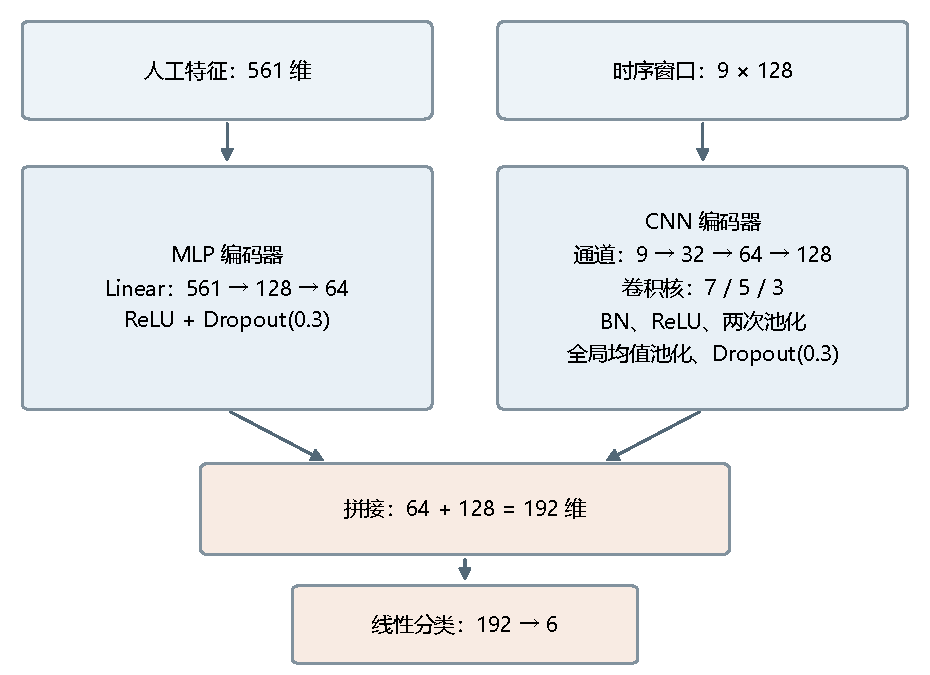
\includegraphics[width=\linewidth]{architecture.pdf}
\caption{双分支融合网络。人工特征与时间序列来自同一窗口；拼接表示维数为 192。}\label{fig:architecture}
\end{figure}
